\section{问题二：床面临界条件与多尺度触发评估}
\subsection{问题定义与适用边界}
水源异常与床面能否起动不是同一命题。本文把连续水力型沟道与冰崩链分开：前者用无黏聚、无超孔压的饱和松散床层给出门槛；后者在现有资料下输出条件状态，不用一次事件的时间窗反向标定系数。附件6的84个对象均为已发生灾点，不含确证非灾沟道，因此本文比较已发生对象之间的门槛和规模，不估计发生概率、真实空间AUC或误报率。

床层竖直厚度记为$z_b$，水深垂直床面，应力和门槛统一按单位坡面面积报告。取水密度$\rho_w=1000\ \mathrm{kg/m^3}$、固相密度$\rho_s=2650\ \mathrm{kg/m^3}$和床体固相体积分数$C_v^{(b)}$，有
\begin{equation}
\rho_{\mathrm{sat}}=C_v^{(b)}\rho_s+(1-C_v^{(b)})\rho_w,
\qquad
\Delta\rho=\rho_{\mathrm{sat}}-\rho_w=1650C_v^{(b)}.
\end{equation}
若$C_v^{(b)}\notin(0,1]$、$\Delta\rho\le0$、$z_b\le0$或比降无效，力学分支记not\_evaluable，不用零密度差继续产生正门槛。

\subsection{完整受力、临界链条与三个分支}
令$S=\tan\theta$。水流在床面产生的拖曳应力、床体沿坡自重和有效法向摩擦抗力分别为
\begin{equation}
\tau_w=\rho_wgh\sin\theta,\qquad
\tau_{g,\parallel}=\Delta\rho\,gz_b\sin\theta\cos\theta,\qquad
\tau_r=\Delta\rho\,gz_b\cos^2\theta\tan\varphi.
\end{equation}
最低无黏聚、无超孔压模型的起动条件为
\begin{equation}
\tau_w+\tau_{g,\parallel}\ge\tau_r.
\end{equation}
控制水流状态时，水流所需承担的净抗力为
\begin{equation}
\tau_{wc}=\Delta\rho\,gz_b\cos^2\theta
\left(\tan\varphi-\tan\theta\right).
\label{eq:tauwc}
\end{equation}
取无量纲容差$\varepsilon_S=10^{-6}$，按$S$与$\tan\varphi$的关系划分：
\begin{equation}
\begin{cases}
\text{水流控制},&S<\tan\varphi-\varepsilon_S,\\
\text{摩擦平衡},&|S-\tan\varphi|\le\varepsilon_S,\\
\text{重力失稳},&S>\tan\varphi+\varepsilon_S.
\end{cases}
\end{equation}
因此$S>\tan\varphi$为重力失稳，零水流门槛不等于安全；$S=\tan\varphi$为摩擦平衡，表示净水流抗力为零，同样不属于“稳定”或“已触发”状态。水流控制时，临界水深、单宽临界流量和断面临界流量依次为
\begin{equation}
h_c=\frac{\tau_{wc}}{\rho_wg\sin\theta},\qquad
q_c=\frac{h_c^{5/3}S^{1/2}}{n_m},\qquad
Q_c=q_c\frac{B}{\kappa_B},
\label{eq:qcrit}
\end{equation}
其中$n_m$为Manning糙率，$B$为全沟宽，$\kappa_B$为全沟宽与有效过流宽度之比。零门槛分支令$h_c=q_c=Q_c=0$，并保留其机械状态；只有水流控制且$Q_c>0$时才定义有限触发比$T=Q_w/Q_c$，避免零除和无意义的无穷大。

基准参数取$C_v^{(b)}=1050/1650=0.636364$、$z_b=1.0$ m、$\tan\varphi=0.55$、$n_m=0.06\ \mathrm{s/m^{1/3}}$、$\kappa_B=6$。中心线沟宽按$B=\min\{9\sqrt{A_{km^2}},400\}$ m取为256.881 m。正式中心线比降为0.10185，代入上式得$h_c\approx4.596$ m、$q_c=67.587745\ \mathrm{m^2/s}$、$Q_c\approx2.893667\times10^3\ \mathrm{m^3/s}$。这些是带明示工程参数的模型门槛，不是现场设防标准。由式\ref{eq:qcrit}可见，$q_c$随$z_b$和$\Delta\rho$按约$5/3$次幂放大，随$n_m$近似反比变化；一次事件不能分别识别床厚、摩擦角、宽度和糙率。

对84条历史沟道，正式状态为78条水流控制、6条重力失稳，无摩擦平衡和不可评估对象。78条正门槛沟道的总起动流量中位为63.261 m$^3$/s，四分位区间为12.614--228.441 m$^3$/s。床体固相分数取0.15、0.636364、0.80时，正门槛中位分别约5.690、63.261、92.635 m$^3$/s，说明床体密度假设本身可改变门槛量级。图\ref{fig:q2-critical}给出完整受力分支、正门槛分布和参数敏感性。

\begin{figure}[htbp]\centering
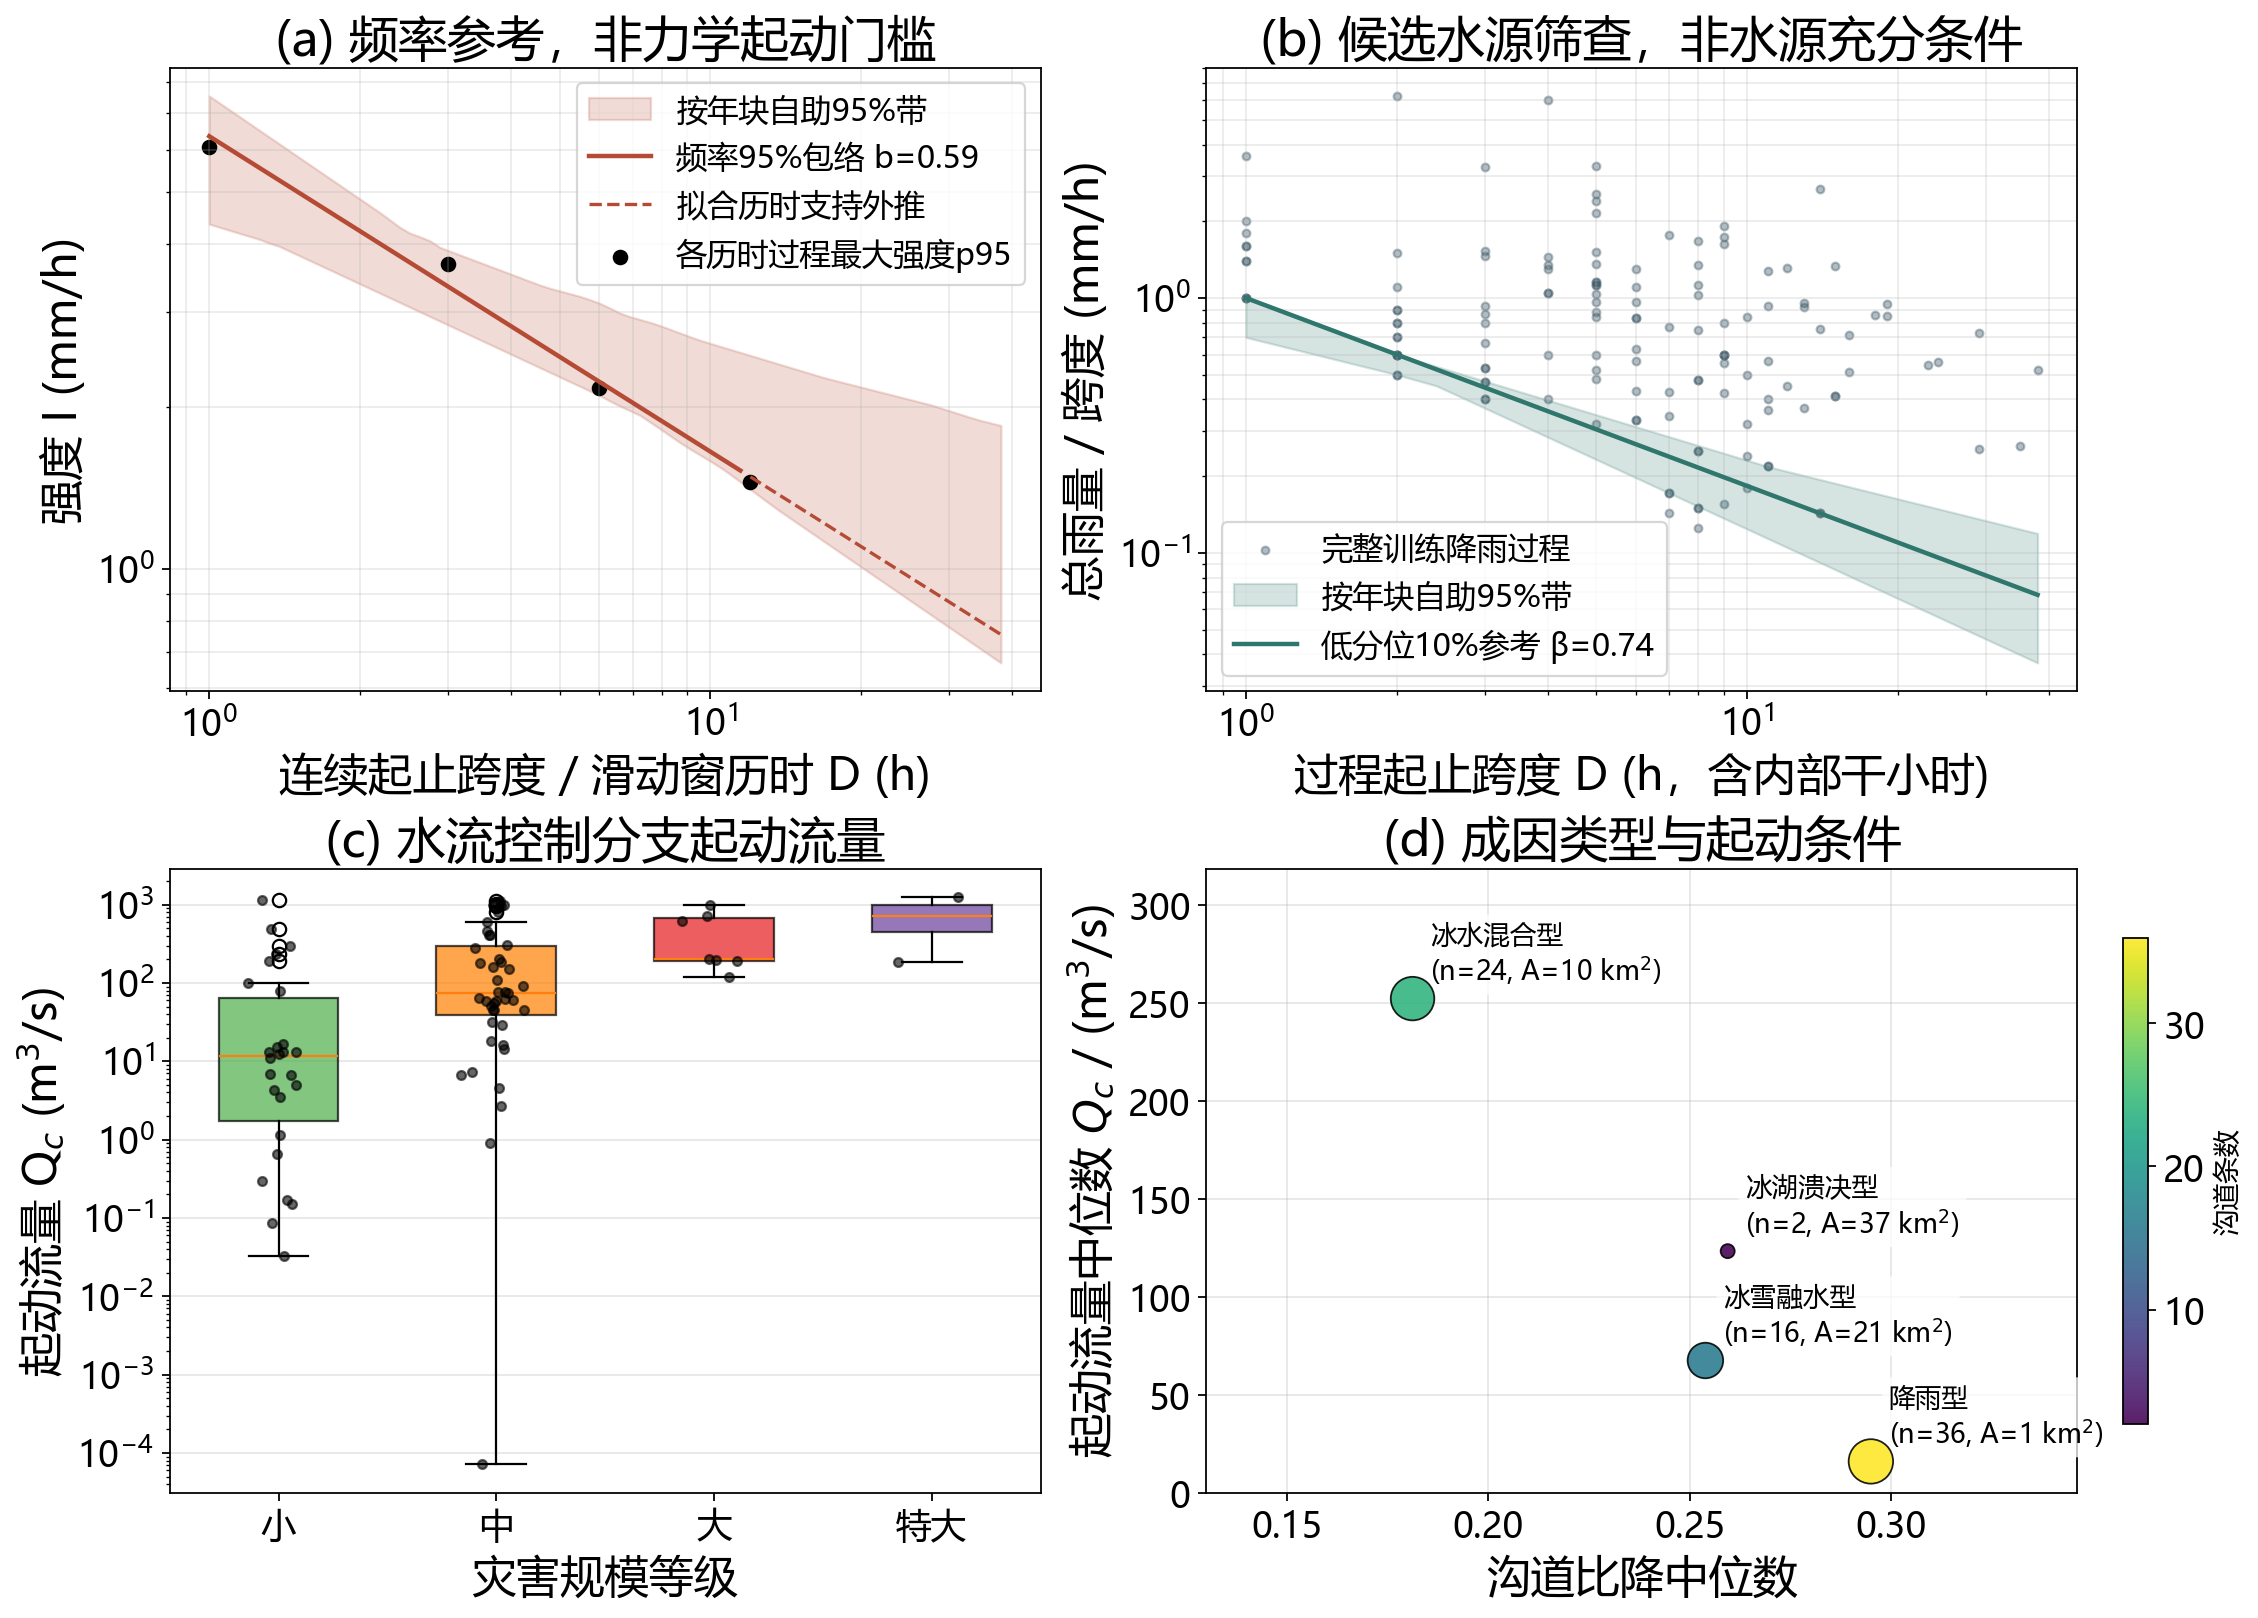
\includegraphics[width=0.80\textwidth]{figures/02_临界条件.png}
\caption{临界条件与参数敏感性}
\label{fig:q2-critical}
\end{figure}

\subsection{对象级状态元组与冰崩链状态识别}
84个对象以源数据唯一标识object\_id存储，不使用可重复的显示名称作为主键。每个对象和时刻保存六元组
\begin{equation}
\mathcal R_j=(G_j,H_j,\Theta_j,F_{\mathrm{ice},j},U_{\mathrm{ice},j},C_{\mathrm{ice},j}),
\end{equation}
其中$G$为水流控制、摩擦平衡、重力失稳或不可评估；$H$为水力候选、低于门槛、不适用或不可评估；$\Theta$为热力前兆成立、低于热力参照或不可评估。$F_{\mathrm{ice}}$表示附件4中存在冰厚与坡度同时达到源区阈值的编目像元，本数据中阈值为50 m与25$^\circ$，共335个像元；$U_{\mathrm{ice}}$记录冰体强度、裂隙、位移或监测资料缺失；$C_{\mathrm{ice}}$只在热力前兆成立且$F_{\mathrm{ice}}=1$时为1。

事件时刻将同一口岸集水区水源流量施加于84个历史沟道几何作比较，$H$的计数为44条低于门槛、34条水力候选、6条不适用。该统计是同一流量口径下的条件对照，不是84条沟道在现场同时获得相同水源的观测事实。事件日$\Theta$为低于热力参照，因而对象层$C_{\mathrm{ice}}=0$；但$U_{\mathrm{ice}}=1$表明冰体力学状态仍不可识别，该保留项始终存在。热力未达参考、有限水力比未越1，均不能证明冰体没有失稳，也不能把状态元组压成未经校准的0--1概率。

\subsection{水源流量与事件前处理}
SCS-CN是单场降雨的累计损失模型，初损按完整事件累计，不逐小时重置\cite{hawkins2009}。对完整小时轴，连续六个已观测、严格零降雨小时确认事件边界；短于六小时的干隙保持同一事件，微量正降雨仍属于降雨，不套用I--D筛查的湿小时阈值。设事件起始小时为$s_e$，事件累计雨量为$P_e(t)=\sum_{u=s_e}^{t}P(u)$，累计直接径流曲线与逐时增量为
\begin{equation}
F_e(P)=
\begin{cases}
\dfrac{(P-I_{a,e})^2}{P-I_{a,e}+S_e},&P>I_{a,e},\\[2mm]
0,&P\le I_{a,e},
\end{cases}
\qquad
R_{\mathrm{rain}}(t)=F_e(P_e(t))-F_e(P_e(t-1)),
\label{eq:scs}
\end{equation}
其中$P_e(s_e-1)=0$，$S_e=25400/C_{N,e}-254$，$I_{a,e}=0.2S_e$。单场内初损只扣一次；事件起始前的最后一小时记为$s_e-1$。基准曲线数$C_{N,0}=85$是独立设定的工程情景，不由土地覆盖类码推导。API分位只用2021--2025年6--9月的14640个有效小时计算，固定为$q_1=3.574888$、$q_3=10.194567$；不使用全季节回退，也不用2026年重估。场初曲线数由事件起始前一小时的API确定：
\begin{equation}
C_{N,e}=\operatorname{clip}
\begin{cases}
0.75C_{N,0},&\mathrm{API}(s_e-1)<q_1,\\
C_{N,0},&q_1\le \mathrm{API}(s_e-1)\le q_3,\\
1.15C_{N,0},&\mathrm{API}(s_e-1)>q_3,
\end{cases}
\quad[30,98].
\end{equation}
事件内不再随API改变而重新套用累计公式作差。初始边界、时间缺口或缺测降雨使累计状态未知，须重新观测到六个连续严格零雨小时才恢复已知边界；负雨量和非有限值视为无效，不将负值裁零来制造干期。若场初前一小时API不可用，整个事件的正雨产流记不可评估；已知场初且记录末端未闭合的事件，其已观测前缀仍可计算。汇流继续按原核传播缺测，缺测保持为空。该分级与六小时边界近似前期含水量和事件分隔，缺少本区水文率定；三、六、十二小时边界的函数行为已由单元测试核对。

源区温度由站点温度按0.006 K/m直减率外推至有效冰厚像元平均高程5109.653 m，站点高程取3980 m，温差订正为$-6.7779\ ^\circ$C。融水权重取Logistic温度因子$w_T(t)$\cite{hock2005}，RGI6编目边界与集水区面积交比$f_{gl}=0.23602$。于是
\begin{equation}
m_{\mathrm{src}}(t)=\frac{w_T(t)e_m(t)}{0.334},\qquad
m_{\mathrm{cat}}(t)=f_{gl}m_{\mathrm{src}}(t),
\end{equation}
其中$e_m$以MJ/(m$^2\cdot$h)计，0.334 MJ/m$^2$对应1 mm水当量。雨与融水分别作三小时汇流后，
\begin{equation}
Q_w(t)=\frac{A_{km^2}}{3.6}\left[
\sum_{i=0}^{2}w_iR_{\mathrm{rain}}(t-i)
+\frac13\sum_{i=0}^{2}m_{\mathrm{cat}}(t-i)\right],
\quad
(w_0,w_1,w_2)=(0.6,0.3,0.1).
\label{eq:water}
\end{equation}
$f_{gl}$是编目年代面积权重，不是2026年实时冰雪范围；任一必需小时缺测时，$Q_w$保持缺测。

\subsection{事件窗求解与水力状态}
正式事件窗为2026年8月26日08:00--13:00的六个整点标签。水源窗峰值为202.650179 m$^3$/s，出现在13:00；相对正式中心线门槛，触发比在该时为
\begin{equation}
T_{\mathrm{peak}}=\frac{202.650179}{2.893667\times10^3}
=0.07003232034381977,
\end{equation}
10:00的$T=0.018814$，窗口内$T\ge1$的小时数为0，未出现越阈时刻。该结果说明当前无黏聚、无超孔压水控链条没有把此次冰崩链识别为水力越阈事件；它不说明冰体未失稳，反而要求保留$U_{\mathrm{ice}}=1$的冰力学未识别状态。旧事件窗标定系数$k=11.19431$仅作对照，正式模型不使用事件窗$k$，也不将窗口水源峰值归一为1。

\begin{figure}[htbp]\centering
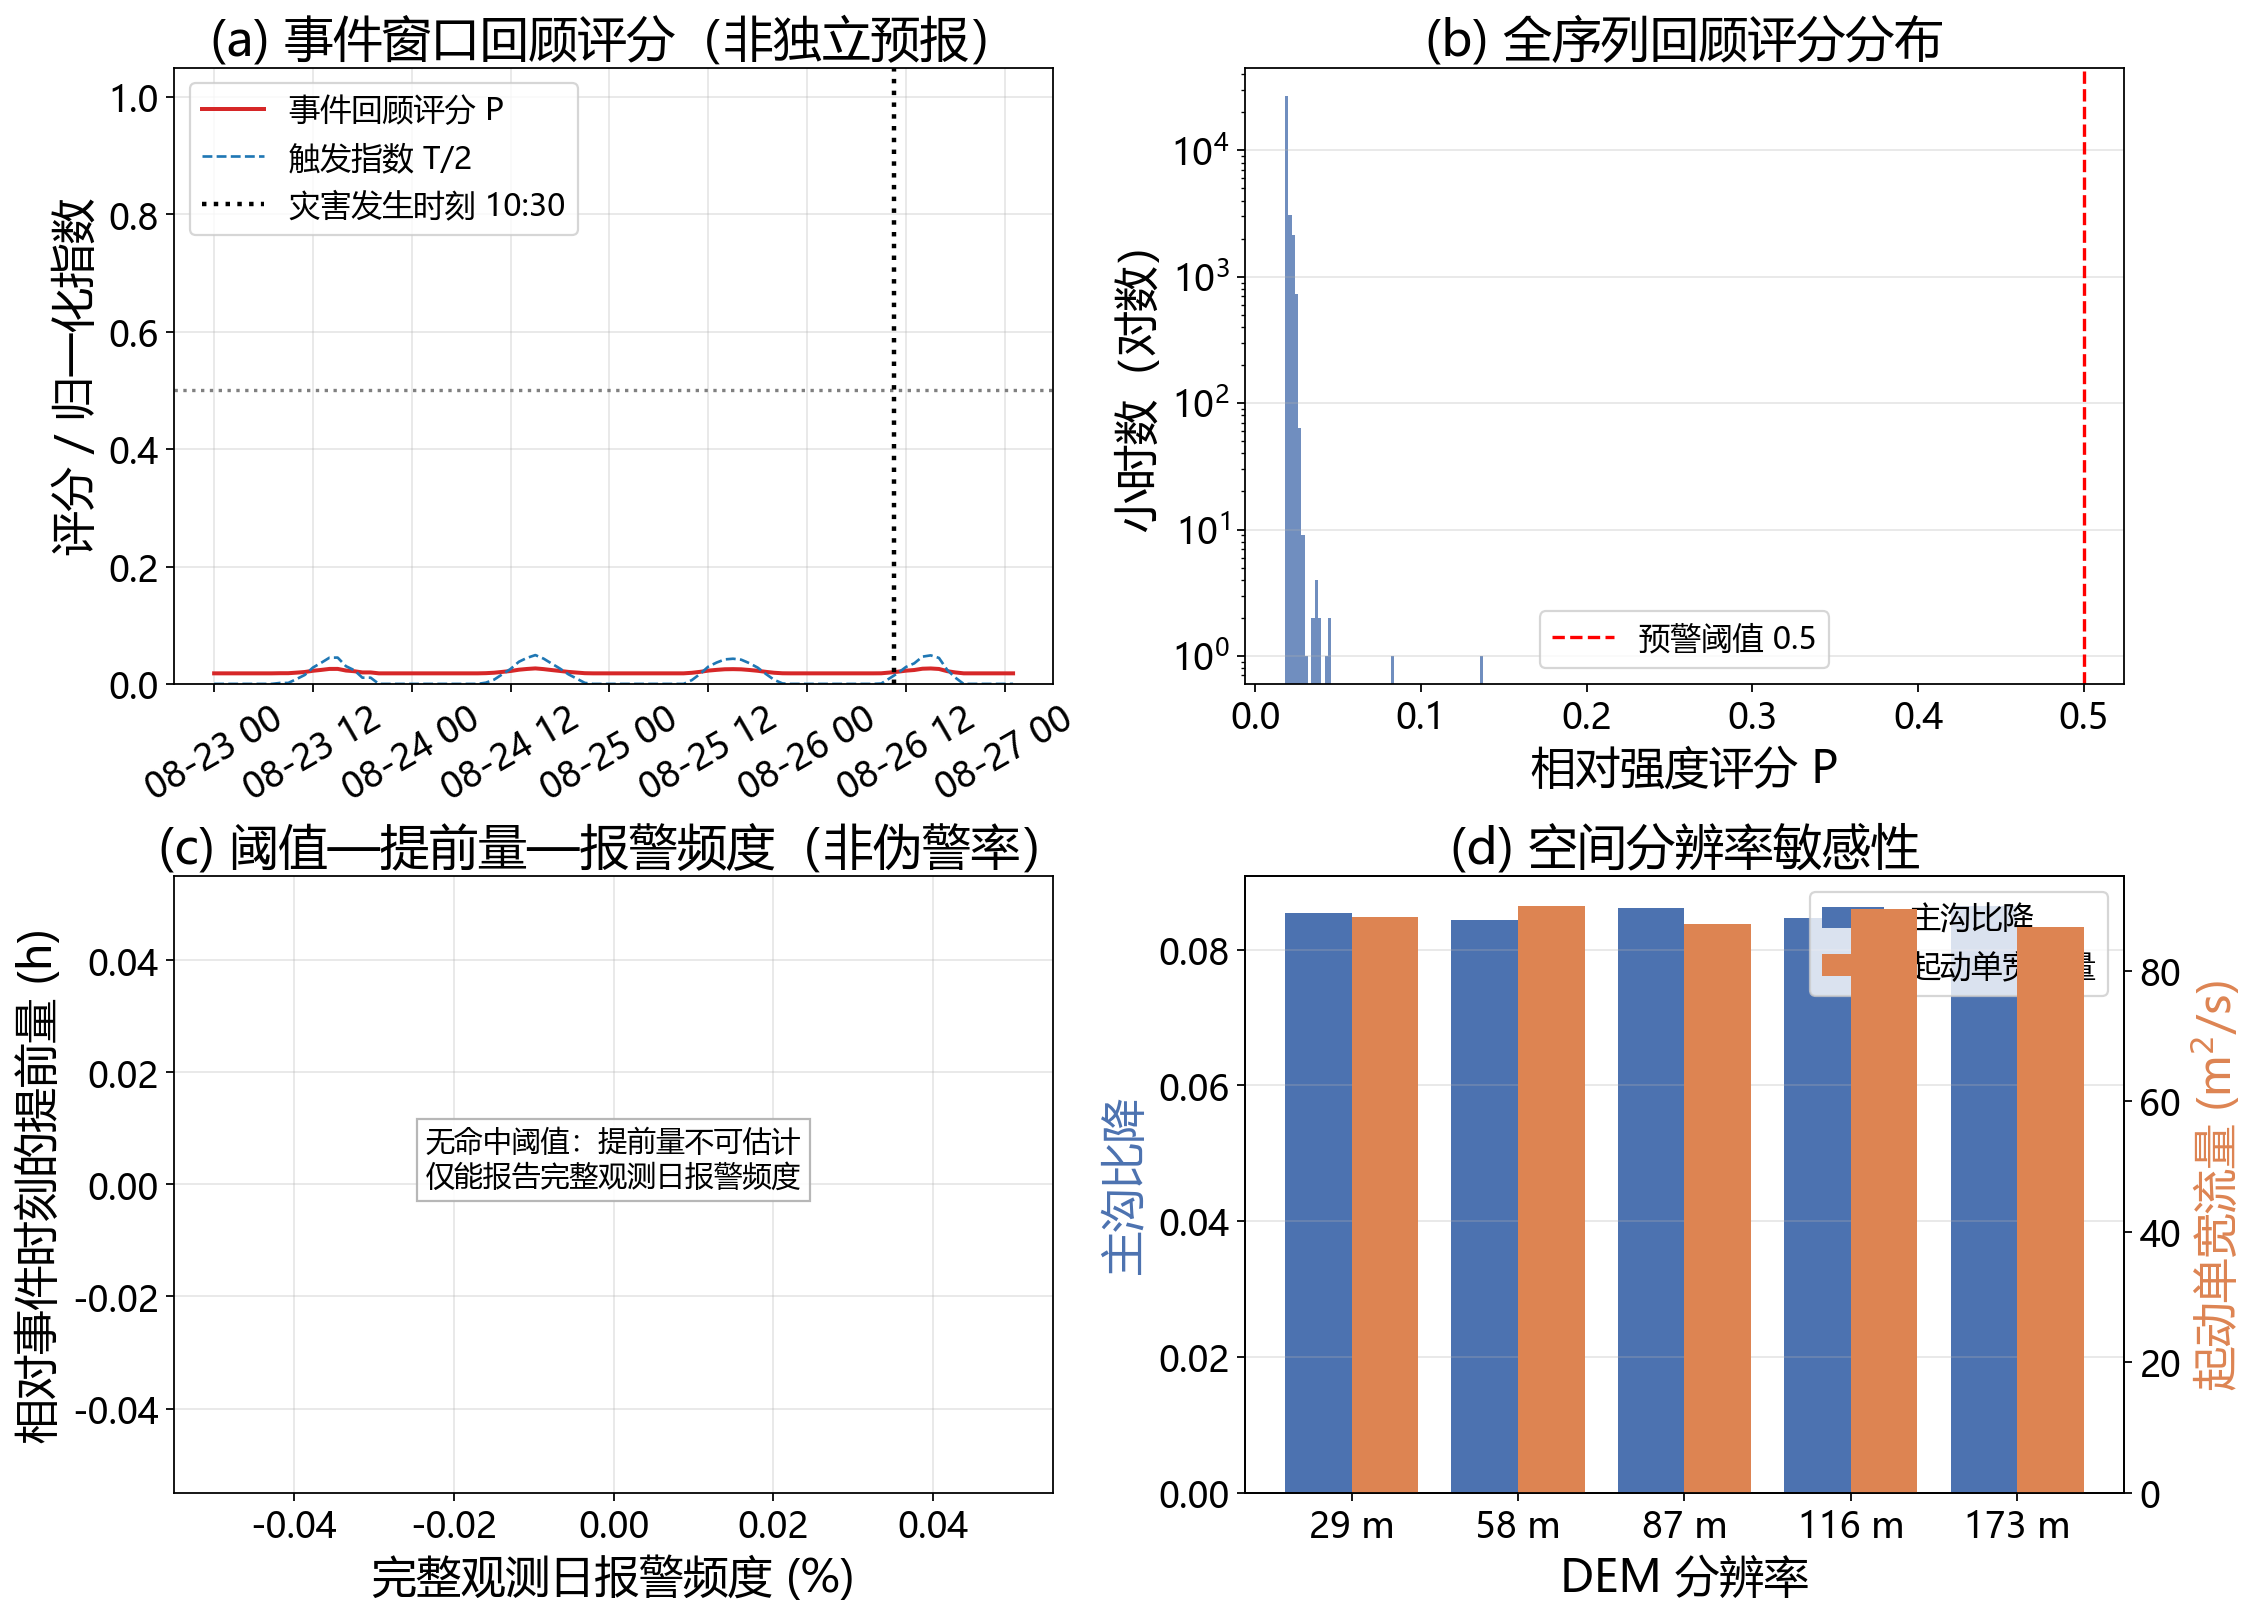
\includegraphics[width=0.80\textwidth]{figures/02_触发评估.png}
\caption{水源流量与触发比}
\label{fig:q2-trigger}
\end{figure}

图\ref{fig:q2-trigger}把事件窗与更长时间序列放在同一条件门槛下展示；图中$T$是条件强度比，不是发生概率，事件窗内未出现$T\ge1$。未越阈是当前模型的结果，不是对冰体失稳或链式过程发生的否定。

\subsection{历史规模关联与双语义降雨包络}
在78条水流控制正门槛对象上，分别检验总起动流量$Q_{\mathrm{crit}}=q_{\mathrm{crit}}B/\kappa_B$和单宽起动流量$q_{\mathrm{crit}}$与已发生对象规模排序的关系，二者名称与量纲需分开。总流量对规模的Kendall检验为$\tau=0.408386$、$p=5.471436410144295\times10^{-6}$，Spearman检验为$\rho=0.498676$、$p=3.3745699520687622\times10^{-6}$；单宽流量对规模的Kendall检验为$\tau=0.318602$、$p=3.904720246143714\times10^{-4}$，Spearman检验为$\rho=0.400620$、$p=2.784782801479891\times10^{-4}$。四组$p$值均按双精度和科学计数法保留，不静默舍入为零。正相关表明在本已发生对象中，较大规模沟道并不具有更低的流量门槛；它不支持发生概率方向，也不能外推到未发生沟道。

降雨阈值保持两种语义\cite{guzzetti2008}。138场完整降雨过程给出的95\%频率包络为$I_{95}(D)=6.3507D^{-0.5853}$，事件平均强度的10\%分位参考为$I_{10}(D)=1.0000D^{-0.7374}$，$D$以小时计、$I$以mm/h计。前者描述历史稀有度，后者只是未作灾害标注的低分位候选筛查线；二者含义不同，不取平均；“超过包络”只表示历史稀有，不表示真实起动。完整样本支持到12小时，更长时间的幂律仅作外推提示。

\subsection{时间与空间可靠性}
时间聚合按同一有效窗比较。3、6小时和日尺度的有效窗口数分别为10583、4980、1190，平均/峰值保持率为0.722655、0.537989、0.230808；三种聚合下均无$T\ge1$窗口。2021--2026年最大$T$分别为0.136392、0.195132、0.104129、0.540807、0.397600、0.235953，均明显低于1。全序列触发评分$P$的最大值为0.137433，出现在2024-09-28 18:00，也远低于0.5的报文门槛。平均会削弱短脉冲，但本数据中即使取窗内峰值也未越阈；该负值反映当前参数与分辨率下的模型行为，不表示现场未发生链式过程。

继承像元对照在30、90、270米名义尺度上的LR AUC分别为0.9814、0.9269、0.8790，组块自举区间分别约为$[0.9757,0.9872]$、$[0.8984,0.9571]$、$[0.8355,0.9195]$。这些数值主要反映灾点面内正像元与面外500米背景的采样环境差异；背景没有确证非灾真值，不代表发生概率或危险区划。共同候选域统一DEM、覆被、最小地面面积和500米隔离后，三尺度均只形成2个正组和188个背景组，无法形成至少两折同时含两类的训练/测试划分，因此不报告AUC。图\ref{fig:q2-common-domain}展示共同域、物理块和空间隔离的诊断结果。

\begin{figure}[htbp]\centering
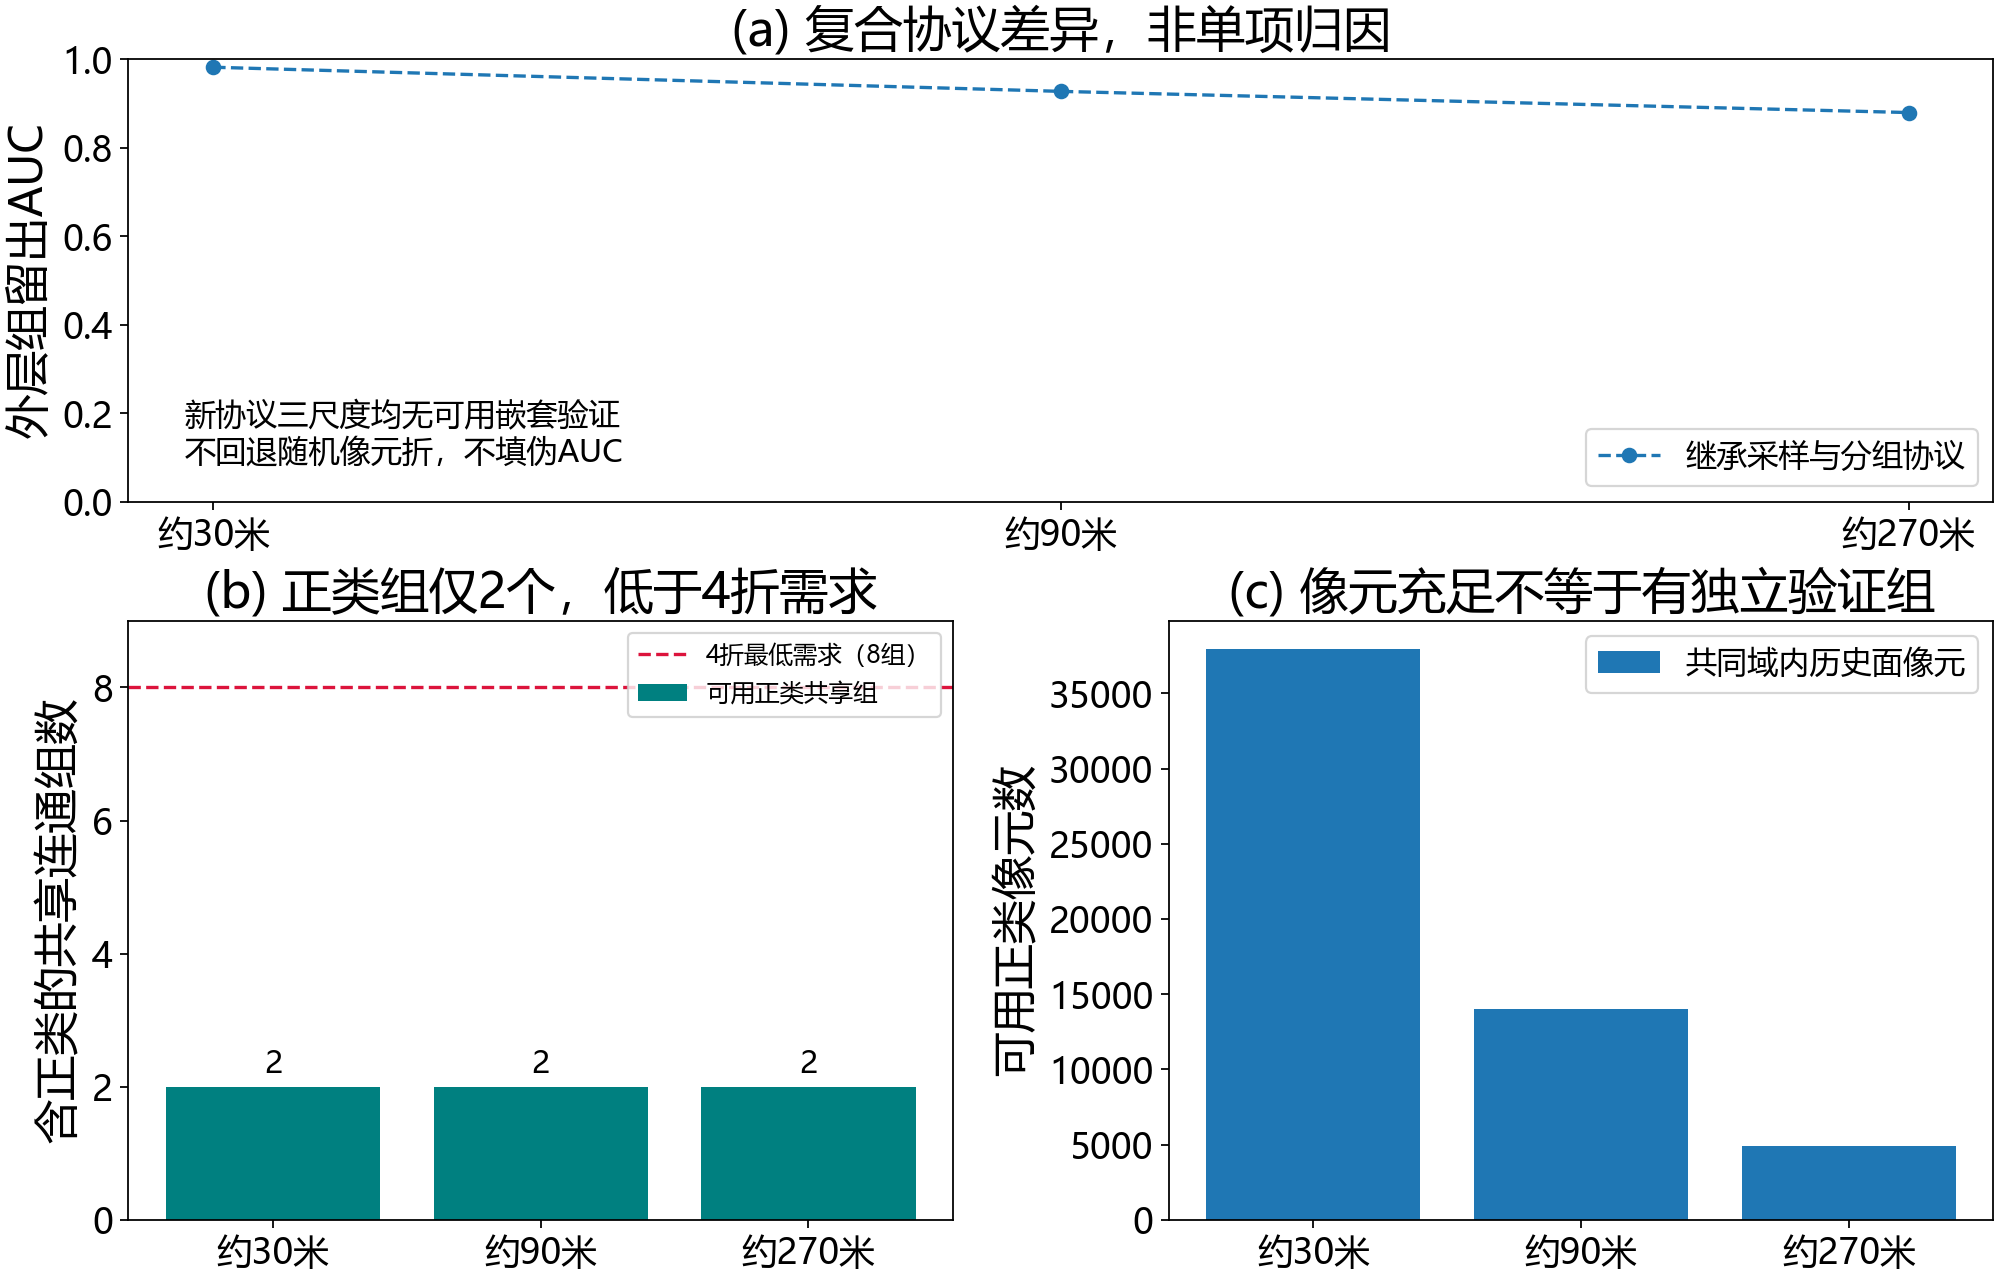
\includegraphics[width=0.92\textwidth]{figures/02c_共同域空间隔离.png}
\caption{共同域空间隔离诊断}
\label{fig:q2-common-domain}
\end{figure}

分辨率和路径口径也会改变门槛。用于D8追迹敏感性检验的主沟比降在2--6倍粗化下为0.084354--0.086502，单宽临界流量约86.699--89.999 m$^2$/s，集水区面积相对偏差绝对值不超过0.4814\%，但口岸投影偏移最大约83.4 m。上述范围与正式中心线门槛不混作同一口径：前者检验路由和粗化稳定性，后者使用公共注入至口岸中心线。中心线平均比降不覆盖每个局部起动段；跨尺度移植时宽度、汇流和床面材料可能同时变化。

\subsection{综合判读}
正式链条是“床体沿坡自重＋水流拖曳与大有效法向摩擦”的条件力平衡，再经$h_c$、$q_c$、Manning和$Q_c$转换到断面尺度。84条历史沟道中78条仍需正水流门槛、6条在给定模型参数下重力失稳。事件窗中心线水源峰值202.650179 m$^3$/s对应$T_{\max}=0.070032$，10:00仅0.018814，当前水控模型未越阈；冰体源区虽有335个达到50 m/25$^\circ$阈值的像元，但强度、裂隙和位移资料缺失，冰力学状态仍未识别。空间上仅能确认继承采样环境的可分性，严格共同域因正组不足而不可估计；时间上仅能确认水控门槛未越，而水控未越不等于冰崩链未发生。模型适用于有有效几何且床面假设落在给定范围内的条件评估；真实发生概率、无资料沟道安全认证和未经校准的危险区划不在本文范围。
